\documentclass[11pt,a4paper]{report}
\usepackage{fontspec}
\usepackage{multirow}
\defaultfontfeatures{LetterSpace=5}
\setmainfont{Times New Roman}
\usepackage{graphicx}
\usepackage{setspace}
\usepackage[a4paper,right=1in,left=1.5in,top=1in,bottom=1in]{geometry}

% TODO Use this package to link from Contents and Sections
% \usepackage[colorlinks=true,linkcolor=blue]{hyperref}

\makeatletter

\newcommand\frontmatter{%
    \cleardoublepage
  %\@mainmatterfalse
  \pagenumbering{roman}}

\newcommand\mainmatter{%
    \cleardoublepage
 % \@mainmattertrue
  \pagenumbering{arabic}}

\newcommand\backmatter{%
  \if@openright
    \cleardoublepage
  \else
    \clearpage
  \fi
 % \@mainmatterfalse
   }

\makeatother

\begin{document}

\frontmatter

\begin{titlepage}
\begin{center}

\textbf{A Summer Internship Report}

\vspace{1em}

\large \textbf{OVERVIEW OF OFFSHORE TERMINAL OF RIL AT GADIMOGA}

\vspace{3em}

\large \textit{\textbf{A report submitted in partial fulfilment for the award of degree of}}

\vspace{1em}

\textbf{Bachelor of Technology in Petroleum Engineering}

\vspace{3em}

\textit{By}

\vspace{1em}

\textbf{Student Name}
    
\textbf{(Roll no.)}

\vspace{2em}

\textit{Under the Guidance and Supervision of}

\vspace{1em}

\textbf{Guide Name}

\textbf{Designation of Guide}

\textbf{Name of the Industry}

\vspace{2em}


\includegraphics[scale=0.3]{jntuk1}

\vspace{1em}

\doublespacing

\large \textbf{DEPARTMENT OF PETROLEUM ENGINEERING AND \\ 
PETROCHEMICAL ENGINEERING}

\large \textbf{UNIVERSITY COLLEGE OF ENGINEERING KAKINADA (A)}

\large \textbf{JAWAHARLAL NEHRU TECHNOLOGICAL UNIVERSITY KAKINADA}

\large \textbf{KAKINADA – 533003}

\large \textbf{2018}

\end{center}
\end{titlepage}

\newpage

\begin{center}
\section*{DECLARATION}
\end{center}

\vspace{4em}


I, \textbf{KATTA SRIDHAR}, hereby declare that this summer internship report entitled “Drilling Services” is original and has not previously formed the basis for the award of any degree to similar work.


\vspace{5em}

\noindent Place: KAKINADA  \hfill Signature     \hspace{0.02\textwidth}

\vspace{1em}

\noindent DATE: 1-12-2018  \hfill Katta Sridhar


\newpage

\begin{center}
\section*{AKNOWLEDGEMENTS}
\end{center}


\vspace{1em}

I would like to express my profound sense of gratitude to my guide and supervisor, Name, \textbf{Designation, Department, Industry,} for his skillful guidance, timely suggestions and encouragement in completing this project. (Others in industry who helped in the internship program may be mentioned)

\vspace{1em}


I acknowledge my sincere thanks and deep felt gratitude to \textbf{Prof. K.V.Rao}, Programme Director, Petroleum Courses, Jawaharlal Nehru Technological University Kakinada for arranging the summer internship program.

\vspace{1em}

I take this opportunity to express my sincere thanks to \textbf{Dr. K. Meera Saheb}, Head of the Department, Department of Petroleum Engineering and Petrochemical Engineering for encouraging and motivating me to complete the internship and report successfully.

\vspace{1em}

Also I express my special thanks to our beloved Principal, \textbf{Dr. P. Subba Rao} his enthusiastic support in our endeavours.

\vspace{1em}

Finally, I am very much grateful to my parents for their financial support and encouragement throughout the internship programme.

\vspace{1em}

\hfill \textbf{Katta Sridhar}

% TODO Center Roll Number w.r.t Name  
\hfill \textbf{Roll number} \hspace{0.005\textwidth}
        
\newpage        
\tableofcontents



\newpage

\begin{center}
\section*{ABSTRACT}
\end{center}
  
The abstract is to be in fully-justified italicized text, at the top of the left-hand column as it is here, below the author information. Use the word “Abstract” as the title, in 12-point Times, boldface type, centered relative to the column, initially capitalized. The abstract is to be in 10-point, single-spaced type, and may be up to 3 in. (7.62 cm) long. Leave two blank lines after the abstract, then begin the main text. All manuscripts must be in English.
  
\vspace{2em}
  
An Abstract is required for every paper; it should succinctly summarize the reason for the work, the main findings, and the conclusions of the study. The abstract should be no longer than 250 words. Do not include artwork, tables, elaborate equations or references to other parts of the paper or to the reference listing at the end. The reason is that the Abstract should be understandable in itself to be suitable for storage in textual information retrieval systems.
  
\newpage


\listoftables


\newpage


\listoffigures


\newpage

\mainmatter

\newpage



\chapter{ABOUT ONGC}

\onehalfspacing 

Oil and Natural Gas Corporation Limited (ONGC) is an Indian multinational oil and gas company earlier headquartered in Dehradun, Uttarakhand, India. As a Corporation, its registered office is now at Deendayal Uurja Bhavan, Vasant Kunj, New Delhi (110070) India. It is a Public Sector Undertaking (PSU) of the
Government of India, under the administrative control of the Ministry of Petroleum and Natural Gas. It is India's largest oil and gas exploration and production company. It produces around 70\% of India's crude oil (equivalent to around 30\% of the country's total demand) and around 62\% of its natural gas.

\section*{History of ONGC}

\begin{enumerate}

\item Foundation to 1961

\begin{enumerate}[(a)]

\item Before the independence of India in 1947, the Assam Oil Company in the north-eastern 
and Attock Oil Company in north-western part of the undivided India were the only oil producing
companies, with minimal exploration input. The major part of Indian sedimentary basins was 
deemed to be unfit for development of oil and gas resources.

\item After independence, the Central Government of India realized the importance of oil and gas 
for rapidindustrial development and its strategic role in defense.Consequently, while framing 
the Industrial Policy Statement of 1948, the development of petroleum industry in the country 
was considered to be of utmost necessity.

\item In 1955, Government of India decided to develop the oil and natural gas resources 
in the various regions of the country as part of the Public Sector development. 
With this objective, an Oil and Natural Gas Directorate was set up towards the end of 1955,
 as a subordinate office under the then Ministry of Natural Resources and Scientific Research. 
 The department was constituted with a nucleus of geoscientists from the Geological Survey of India.

\item Soon, after the formation of the Oil and Natural Gas Directorate, it became apparent that it would 
not be possible for the Directorate with its limited financial and administrative powers as subordinate 
office of the Government, to function efficiently. So in August, 1956, the Directorate was raised to the
status of a commission with enhanced powers, although it continued to be under the government. 
In October 1959, the Commission was converted into a statutory body by an act of the Indian Parliament, 
which enhanced powers of the commission further. The main functions of the Oil and Natural Gas Commission 
subject to the provisions of the Act, were "to plan, promote, organize and implement programs for 
development of Petroleum Resources and the production and sale of petroleum and petroleum products produced 
by it, and to perform such other functions as the Central Government may, 
from time to time, assign to it ". The act further outlined the activities and steps to be taken 
by ONGC in fulfilling its mandate.

\end{enumerate}


\item From 1961 to present

\begin{enumerate}[(a)]

\item Since its inception, ONGC has been instrumental in transforming the country's limited upstream sector into a large viable playing field, with its activities spread throughout India and significantly in overseas territories. In the inland areas, ONGC not only found new resources in Assam but also established new oil province in Cambay basin (Gujarat), while adding new petroliferous areas in the Assam-Arakan Fold Belt and East coast basins (both onshore and offshore).

\item ONGC became a publicly held company in February 1994, with 20\% of its equity were sold to the public and eighty percent retained by the Indian government. At the time, ONGC employed 48,000 people and had reserves and surpluses worth ₹104.34 billion, in addition to its intangible assets. The corporation's net worth of ₹107.77 billion was the largest of any Indian company .

\item In 2003, ONGC Videsh Limited (OVL), the division of ONGC concerned with its foreign assets, acquired Talisman Energy's 25\% stake in the Greater Nile Oil project.

\item In 2006, a commemorative coin set was issued to mark the 50th anniversary of the founding of ONGC, making it only the second Indian company (State Bank of India being the first) to have such a coin issued in its honor.

\item In 2011, ONGC applied to purchase 2000 acres of land at Dahanu to process offshore gas. ONGC Videsh, along with Statoil ASA (Norway) and Repsol SA (Spain), has been engaged in deep-water drilling off the northern coast of Cuba in 2012. On 11 August 2012, ONGC announced that it had made a large oil discovery in the D1 oilfield off the west coast of India, which will help it to raise the output of the field from around 12,500 barrels per day (bpd) to a peak output of 60,000 bpd.


\begin{table}[H]

\centering

\caption{Product-wise revenue breakup for FY 2016–17 (₹ billion)}

\vspace{1em}

\begin{tabular}{|l|l|lll}
\cline{1-2} 
\textbf{Product}     & \textbf{Revenue} &  &  &  \\ \cline{1-2}
Crude Oil            & 526.38           &  &  &  \\ \cline{1-2}
Gas                  & 168.88           &  &  &  \\ \cline{1-2}
LPG                  & 31.48            &  &  &  \\ \cline{1-2}
Naptha               & 36.80            &  &  &  \\ \cline{1-2}
C2-C3                & 13.44            &  &  &  \\ \cline{1-2}
Others               & 1.59             &  &  &  \\ \cline{1-2}
Adjustments          & -32.74           &  &  &  \\ \cline{1-2}
Total                & 825.52           &  &  &  \\ \cline{1-2}
\multicolumn{2}{|l|}{Rs.825.52 billion} &  &  &  \\ \cline{1-2}
\end{tabular}


\end{table}

\vspace{1em}

\item In November 2012, OVL agreed to acquire ConocoPhillips' 8.4\% stake in the Kashagan oilfield in Kazakhstan for around US\$5 billion, in ONGC's largest acquisition to date. The acquisition is subject to the approval of the governments of Kazakhstan and India and also to other partners in the Caspian Sea field waiving their pre-emption rights.

\item In January 2014, OVL and Oil India completed the acquisition of Videocon Group's ten percent stake in a Mozambican gas field for a total of \$2.47 billion.

\item In June 2015, Oil and Natural Gas Corporation (ONGC) gave a Rs27bn (\$427m) offshore contract for the Bassein development project to Larsen \& Toubro (L\&T).

\item In February 2016, the board of ONGC approved an investment of Rs. 5,050 crores in Tripura for drilling of wells and creation of surface facilities to produce 5.1 million standard cubic feet per day gas from the state's fields.

\item On 19 July 2017, the Government of India approved the acquisition of Hindustan Petroleum Corporation by ONGC.

\vspace{1em}

\end{enumerate}

\end{enumerate}

\noindent Table 1.1 shows the Product-wise revenue breakup for FY 2016–17 (₹ billion) which is shown above.

\vspace{2em}


\noindent ONGC Videsh is a wholly owned subsidiary of Oil and Natural Gas Corporation Limited (ONGC), 
the National Oil Company of India, and is India’s largest international oil and gas Company. 
ONGC Videsh has participation in 41 projects in 20 countries namely Azerbaijan, Bangladesh, Brazil, 
Colombia, Iraq, Israel, Iran, Kazakhstan, Libya, Mozambique, Myanmar, Namibia, Russia, South Sudan, Sudan,
Syria, United Arab Emirates, Venezuela, Vietnam and New Zealand. ONGC Videsh maintains 
a balanced portfolio of 15 producing, 4 discovered/under development, 18 exploratory and 4 pipeline projects. 
The Company currently operates/ jointly operates 21 projects. ONGC Videsh had total oil and gas reserves (2P) 
of about 711 MMTOE as on April 1, 2018.





\chapter{About Mehsana Asset}

The Mehsana Tectonic Block is a fairly well explored, productive hydrocarbon block of North Cambay Basin. Exploration activity for hydrocarbons by ONGC in the Mehsana Asset commenced in the 1960s and discovered fields are in an advanced stage of exploitation. The Asset has been endowed with a number of oil fields with multilayered pays belonging to Paleocene to middle Miocene age.More than 26 small to medium size oil and gas fields have been established in the Mehsana area of Mehsana-Ahmedabad Tectonic Block.Operational areas for the Mehsana Asset include a Mining Lease(ML) area of 942 Km 2 . In this Asset, 2324 wells have been already
drilled. Further, 35 production installations have already been established to complete the hydrocarbon production, storage and delivery cycle. The Asset currently produces 6100 TPD of crude oil and 5 Lakh m 3 of natural gas on a daily basis.

Major oil fields within the Asset have been clubbed under six different areas:

1. Becharaji \& Lanwa (Area-I)

2. Sathal \& Balol (Area-II)

3. Jotana (Area-III)

4. Sobhasan Complex (Area- IV)

5. Nandasan, Linch, Langhnaj, Mansa \& other satellite structures (Area-V), and

6. North Kadi (Area-VI)

Area I \& II constitute the heavy oil fields of the Mehsana Asset.

The Asset, spread over four districts in North Gujarat, covers:

Two talukas of Patan and Ahmedabad Districts Six talukas in Mehsana District,and One taluka in Gandhinagar District

\section{\textbf{The Drilling Process}}

Drilling operations shall be conducted round-the-clock for 24 hrs. The time taken to drill a well depends on the depth of the hydrocarbon bearing formation and the geological conditions.ONGC intends to drill wells to a depth range from 1200 to 2000 m. This would typically take ~30 - 35 days for each well – however drilling period may increase depending on well depth.In general, a 17 1⁄2” hole is drilled from the surface up to a predetermined depth and 13 3/8” surface casing is done to cover fresh water sands, prevent caving, to cover weak zones \& to provide means for attaching well head \& the blowout preventer(BOP).This is followed by drilling of 12 1⁄4” hole and lowering of 9 5/8” intermediate casing depending upon the depth of the well and anticipated problems in drilling the well. The 8 1⁄2” holes is drilled up to the target depth of the well cased with 5 1⁄2” or 7” production casing to isolate the producing zone from the other formations.

In the process of drilling, drilling fluid is used to lift the cutting from the hole to the surface. Drilling fluid is formulated by earth clay and barites. Various types of bio-degradable polymers are also added to maintain the specific parameters of the mud. After completion of production casing the well is tested to determine \& analyze various parameters of producing fluid.

Water based mud, that is ecologically sensitive, will be used and all drilling activities will be conducted as per the requirements of the Oilfield and Mineral Development Rules, 1984 as amended till date. Guidelines issued by the Oil Mines Regulation (OMR) will be followed throughout the drilling process.

The power required for driving the drilling rig, circulation system and for providing lighting shall be generated by DG sets attached with the rig deployed by ONGC from various rigs available with ONGC mentioned in the table.. Fuel used in DG sets shall conform to Bharat Stage IV norms including a sulphur content of <50 mg/kg.


\newpage

\begin{table}
\centering
\caption{Power Distribution Table}

\begin{tabular}{|l|l|l|l|}
\hline
Serial no           & \multicolumn{1}{c|}{Rig}                                                                                   & packager    & KVA \\ \hline
\multirow{2}{*}{1.} & \multicolumn{1}{c|}{\multirow{2}{*}{\begin{tabular}[c]{@{}c@{}}IPS-700-V\\ (Mechanical rig)\end{tabular}}} & Sudhir DG   & 500 \\ \cline{3-4} 
                    & \multicolumn{1}{c|}{}                                                                                      & Caterpillar & 438 \\ \hline
\multirow{2}{*}{2.} & \multicolumn{1}{c|}{\multirow{2}{*}{\begin{tabular}[c]{@{}c@{}}IPS-700-V\\ (Mechanical rig)\end{tabular}}} & Sudhir DG   & 500 \\ \cline{3-4} 
                    & \multicolumn{1}{c|}{}                                                                                      & Caterpillar & 438 \\ \hline
\multirow{2}{*}{3.} & \multicolumn{1}{c|}{\multirow{2}{*}{\begin{tabular}[c]{@{}c@{}}IPS-700-V\\ (Mechanical rig)\end{tabular}}} & Sudhir DG   & 500 \\ \cline{3-4} 
                    & \multicolumn{1}{c|}{}                                                                                      & Caterpillar & 438 \\ \hline
\multirow{2}{*}{4.} & \multicolumn{1}{c|}{\multirow{2}{*}{\begin{tabular}[c]{@{}c@{}}IPS-700-V\\ (Mechanical rig)\end{tabular}}} & Sudhir DG   & 500 \\ \cline{3-4} 
                    & \multicolumn{1}{c|}{}                                                                                      & Caterpillar & 438 \\ \hline
\multirow{2}{*}{1.} & \multicolumn{1}{c|}{\multirow{2}{*}{\begin{tabular}[c]{@{}c@{}}IPS-700-V\\ (Mechanical rig)\end{tabular}}} & Sudhir DG   & 500 \\ \cline{3-4} 
                    & \multicolumn{1}{c|}{}                                                                                      & Caterpillar & 438 \\ \hline
\multirow{2}{*}{1.} & \multicolumn{1}{c|}{\multirow{2}{*}{\begin{tabular}[c]{@{}c@{}}IPS-700-V\\ (Mechanical rig)\end{tabular}}} & Sudhir DG   & 500 \\ \cline{3-4} 
                    & \multicolumn{1}{c|}{}                                                                                      & Caterpillar & 438 \\ \hline
\multirow{2}{*}{1.} & \multicolumn{1}{c|}{\multirow{2}{*}{\begin{tabular}[c]{@{}c@{}}IPS-700-V\\ (Mechanical rig)\end{tabular}}} & Sudhir DG   & 500 \\ \cline{3-4} 
                    & \multicolumn{1}{c|}{}                                                                                      & Caterpillar & 438 \\ \hline
\multirow{2}{*}{1.} & \multicolumn{1}{c|}{\multirow{2}{*}{\begin{tabular}[c]{@{}c@{}}IPS-700-V\\ (Mechanical rig)\end{tabular}}} & Sudhir DG   & 500 \\ \cline{3-4} 
                    & \multicolumn{1}{c|}{}                                                                                      & Caterpillar & 438 \\ \hline
\multirow{2}{*}{1.} & \multicolumn{1}{c|}{\multirow{2}{*}{\begin{tabular}[c]{@{}c@{}}IPS-700-V\\ (Mechanical rig)\end{tabular}}} & Sudhir DG   & 500 \\ \cline{3-4} 
                    & \multicolumn{1}{c|}{}                                                                                      & Caterpillar & 438 \\ \hline
\multirow{2}{*}{1.} & \multicolumn{1}{c|}{\multirow{2}{*}{\begin{tabular}[c]{@{}c@{}}IPS-700-V\\ (Mechanical rig)\end{tabular}}} & Sudhir DG   & 500 \\ \cline{3-4} 
                    & \multicolumn{1}{c|}{}                                                                                      & Caterpillar & 438 \\ \hline

\multirow{2}{*}{2.} & \multirow{2}{*}{}                                                                                          &             &     \\ \cline{3-4} 
                    &                                                                                                            &             &     \\ \hline
\end{tabular}
\end{table}


\section{\textbf{Water Requirement}}

The drilling operation and maintenance of the drill site facilities have various water requirements. The most significant of these requirements in terms of quantity is that for mud preparation. The other requirements would be for engine cooling, floor / equipment / string washing, sanitation, fire-fighting storage / make-up and
drinking. Water for emergency fire fighting would be stored in a pit of 200 m 3 capacity and make-up of the same will have to be made on a regular basis.The requirement of water expected for sanitation and drinking purposes of the workers shall be insignificantly low in terms of quantity. ONGC has planned to meet the requirement of water at the drilling site through water supplied by tankers and sourced from nearest ONGC installation. Since, there is no quality criterion for usage of raw water for the various uses mentioned above (other than drinking), the tanker water shall be directly used without any treatment.The potable water requirement shall be met by procuring adequately treated water from off-site locations.

\section{\textbf{Waste Water Generation}}

The drilling operation would generate waste water in the form of wash water due to washing of equipment, string etc. This waste water along with spill over mud will be diverted to waste water mud pit whose bottom would be lined with HDPE sheet so as to avoid percolation of water contaminants in the soil. Approximately 25 m 3 per day of waste water will be discharged in HDPE lined evaporation pit. The domestic sewage generated from the drill site operations will be treated in a septic tank–soak pit system. The septic tank is adequately sized to cater to a volumetric capacity of 4–5 m 3 per day.

\section{\textbf{Air Emissions}}

The emissions to the atmosphere from the drilling operations shall be from the diesel engines and flaring of associated gas during testing operation in case of hydrocarbon is discovered. In accordance with the Oil Mines Regulations Rules, a flare stack of 9m height will be provided.

\section{\textbf{Solid and Hazardous Waste Management}}

The drilling rig system to be employed for drilling will be equipped for the separation of drill cuttings and solid materials from the drilling fluid. The drill cuttings, cut by the drill bit, will be removed from the fluid by the shale shakers (vibrating screens) and centrifuges and transferred to the cuttings containment area.Once the drilling fluid / mud have been cleaned it will be returned to the fluid tank and pumped down the drill string again.It is estimated that 104 MT of formation cuttings and 650 m 3 of drilling mud will be generated in the form of solid waste, during the drilling operation.

Drill cuttings and drilling mud will be disposed off in accordance with the Gazette Notification dated 30th August 2005 - G.S.R 546(E), Section C ‘Guidelines for Disposal of Solid Waste, Drill Cuttings and Drilling Fluids for Offshore and Onshore Drilling
Operation’. 

Under these guidelines:

Drill cuttings separated from Water Based Mud (WBM) will be properly washed and unusable drilling fluids will be allowed toevaporate in a HDPE lined pit. In case the drill cuttings have oil and grease level in.



\chapter{DRILLING}

Once the geoscientists analyze a prospective oil field and the land is leased,
a well is drilled to obtain more information about the reservoir. 
Not all wells are straight and vertical. Horizontal drilling has become a
 very profitable way to increase production by having the wellbore contacting more of the formation.

\section{Drilling Rig}

A drilling rig is a device used to drill, case and cement oil and gas wells. 
In drilling an oil well different types of rigs are used. The type used will
depend on whether the drilling is being done in sea or on land and also on depth.

\section{Rig Components}
The most important rig components include:
 rig engines, derrick and substructure, hoisting equipment, rotary equipment, mud pumps and BOPs.
 
 
 %figures are to be included in the document.  
 
 \subsection*{Rig Engines:}
 
 Rigs suitable for shallow drilling use two engines and deep drilling is achieved by three to four engines.

\subsection*{Derrick and Substructure:}

A derrick is a four sided structure of sufficient height and strength. The
substructure provides support for the derrick, draw-works and drill string.


\section{Hoisting Equipment}

The main function of hoisting equipment is to get the drill string and 
other necessary equipment in and out of the hole safely and efficiently. 
The main components of hoisting system include draw-works, crown and travelling block, hooks, drilling line.

\vspace{1em}

\subsection*{\textbf{Drawworks:}} This is an assembly of a rotating drum, a series of shafts, 
clutches, chains and gears for changing speed and for reversing.
 It also contains the main brake for stopping the drilling line. 
The drilling line is wound a number of times around the drum, 
the end of the line then passes on the crown and travelling block.

\vspace{1em}

\subsection*{\textbf{Crown block:}} A block located at the top of the derrick and is stationary.
 The crown block provides ameans of taking the drilling line from the hoisting drum to the travelling block.

\vspace{1em}

\subsection*{\textbf{Travelling block:}} It is a diamond shaped block. 
The drilling line is wound continuously on the crown and travelling blocks,
 with the two outside ends being wound on the hoisting drum.

\vspace{1em}

\subsection*{\textbf{Hook:}} It connects the Kelly or topdrive with the travelling block. The hook carries the entire drilling load.

\section{Rotary Equipment}

The main components of Rotary equipment are: Rotary table, Kelly, Swivel.

\subsection*{\textbf{Rotary table:}} The main function of the rotary table is to transfer
 the rotary motion through a master bushing to the Kelly, to drill pipe, and eventually to the drill bit.

\vspace{1em}

\subsection*{\textbf{Kelly:}} The Kelly is the rotating link between the rotary table and the drill string.
 Its main functions are transmits rotation and weight-on-bit to the drillbit, supports the
weight of the drill string and conveys the drilling fluid from the swivel into the drill string.
The Kelly has a hexagonal or square shape cross section. The Kelly is usually 
provided with two safety valves, one at the top and one at the bottom, called upper and lowerKelly cocks,
 respectively. The Kelly cock is used to close the inside of the drill string in the event of a kick.
 
 \vspace{1em}
 
\subsection*{\textbf{Swivel:}} The swivel is installed above the Kelly and its main function 
is to prevent the rotary motion of the Kelly from being transferred to the drilling line. 
 
\vspace{1em}

\subsection*{\textbf{Master bushing:}} It serves two purposes:

    a) Provides engagement of the Kelly drive bushing with the rotary table.

    b) Provides tapered seating for the slips which hold drill pipe in the rotary table.

\vspace{1em}

\subsection*{\textbf{Kelly drive bushing:}} It engages with the master bushing.

\section{Drill String Components}

The main component of the drill string includes drill pipe,
drill collars and accessories like stabilizers and reamers.
 	
\vspace{1em}

\subsection*{\textbf{Drill pipe:}} The main function of the drill pipe is to transmit rotary motion and
drilling mud under high pressure to the drill bit.

\vspace{1em}

\subsection*{\textbf{Drill collars:}} Drill collars are the predominant component of the bottom hoe assembly (BHA). 
It is used to provide weight on bit.

\vspace{1em}

\subsection*{\textbf{Stabilizers:}} Stabilizers are tools placed above the drill bit and along the bottom hole assembly (BHA)
to control hole deviation, dogleg severity and prevent differential sticking. 
They achieve these functions by centralizing and providing extra stiffness to the BHA.

\vspace{1em}


\subsection*{\textbf{Reamers:}} Reamers are usually run immediately behind the bit to provide a gauge hole.


\section{Drilling Bits}

Drill bit crushes the rock under combined action of weight on bit and rotary speed.

\vspace{1em}

\textbf{Roller Cone Bits:} These are made up of three equal-sized cones. Each cone is 
mounted on bearings which run on a pin that forms an integral part of the bit leg.
Nozzles are used to provide constriction in order to obtain high jetting velocities 
necessary for efficient bit and hole cleaning. Mud pumped through the drill string passes 
through the bit pin bore and through the three nozzles,with each nozzle accommodating 
one third of the total flow, if all the nozzles were of the same size.
Figure 3.1 shows the image of Roller Cone Bits.

\vspace{1em}

\begin{figure}[h]
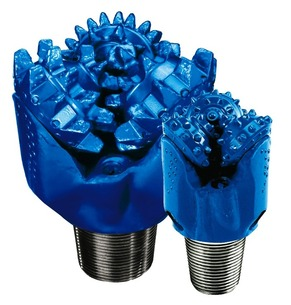
\includegraphics[scale=0.3]{images/Rollerconebits}
\centering 
\caption{A Picture of Roller Cone Bits}
\end{figure}

\textbf{Polycrystalline Diamond Compact Bit:} PDC bit employs no moving parts. 
A PDC bit employs a large number of cutting elements, each called a PDC cutter.The PDC cutter is made 
by bonding a layer of polycrystalline man-made diamond to a cemented tungsten 
carbide substrate in a high pressure, high temperature process. 
The diamond layer is composed of many tiny diamonds which are grown together at random orientation for 
maximum strength and wear resistance.Figure 3.2 shows the image of PDC Bits.

\vspace{1em}

\begin{figure}[h]
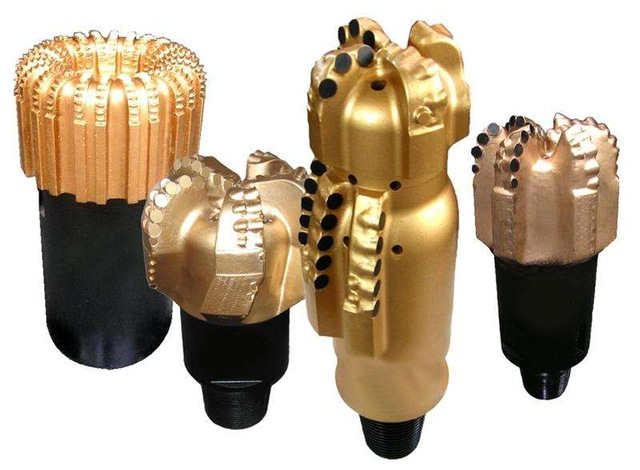
\includegraphics[scale=0.3]{images/PDCbits}
\centering 
\caption{A Picture of PDC Bits}
\end{figure}

\textbf{Diamond Bit:} Diamond is the hardest mineral and also posses the highest thermal conductivity 
of any other mineral allowing it to dissipate heat very quickly. 
These bits are used for drilling hard and
abrasive formations. Diamond bits are manufactured as either drilling or coring bits.



\section{Drilling Mud}
	
Drilling Mud or drilling fluid is a critical component in the rotary drilling processes.

The primary functions of drilling fluids are:

\begin{itemize}

\item Remove cuttings from the wellbore.
\item Prevent formation fluids from entering into the wellbore.
\item Maintain wellbore stability
\item Cool and Lubricate the bit
\item Transmit Hydraulic Horsepower to bit

\end{itemize}

\subsection*{Types of Drilling fluids}

The two major types of mud system used are Oil Based Mud which consists of oil 
as a continuous phase and other is Water Based mud which consists of water as 
a continuous phase.Mostly water based mud is used in Mehsana. The following 
mud systems are in continuous use in Mehsana Asset:

\begin{enumerate}[(a)]

\item SPUD Mud
\item KPPA Mud
\item NDDF Mud

\end{enumerate}

\begin{enumerate}[(a)]

\item \textbf{Spud Mud:}

Mud used to drill a well from the surface to a shallow depth .Onshore spud mud
consists of bentonite clay whereas in offshore guar gum and salt gel are used 
in offshore.

\item \textbf{KPPA Mud:}

It is an abbreviation of KCL, PHPA, polyol mud.KCL and PHPA in the mud acts as 
a shale inhibitor and polyol provides lubricity to the mud.

\item \textbf{NDDF Mud}

It is generally used near pay zone. It is an abbreviation of Non Damaging 
Destructive Fluid which does not uses barite but polymers as a weighing agent as 
barite is non biodegradable and damages the pay zone permeability and porosity.
\end{enumerate}


\noindent \textbf{Field Tests on Drilling Mud}

The mud properties are regularly monitored by mud engineer. These measurements 
will be used to determine if the properties of mud have been deteriorated and 
require treatment or not.

The following tests are used to determine the under mentioned :
\begin{itemize}

\item Mud Density

The density of the drilling mud can be determined with the mud balance shown 
in Figure. The cup of the balance is completely filled with a sample of the
mud and the lid placed firmly on top (some mud should escape through the hole 
in the lid). The balance arm is placed on the base and the rider adjusted until 
the arm is level. The density can be read directly off the graduated scale at 
the left-hand side of the rider.Figure 3.3 shows the image of Mud balance.


\begin{figure}[h]
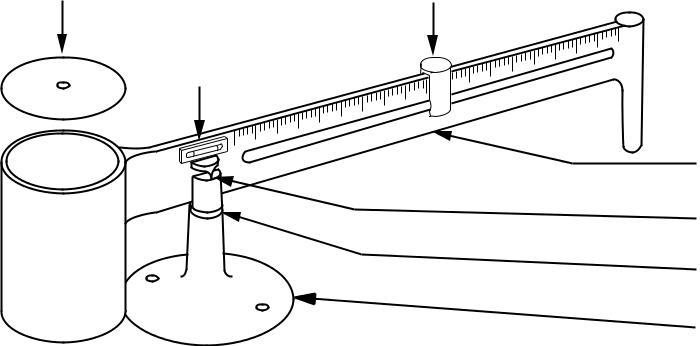
\includegraphics[scale=0.3]{images/mudbalance}
\centering 
\caption{A Picture of Mud Balance}
\end{figure}

\item Viscosity

The rheological character of drilling fluids is discussed at length in the 
chapter on Drilling Hydraulics. In general terms however, viscosity is a 
measure of a liquids resistance to flow. Two common methods are used on the rig 
to measure viscosity.Figure 3.4 shows the image of Marsh Funnel Viscometer.

The marsh funnel viscometer is used to make the quickest analysis of the 
viscosity of drilling fluid .However this device only gives change in 
viscosity and does not quantify rheological properties such as yield point 
and plastic viscosity for which we use rotational viscometer.

Rotational viscometer: The multi-rate rotational viscometer is used
to quantify the rheological properties of the drilling mud. The
assessment is made by shearing a sample of the mud, at a series of
prescribed rates and measuring the shear stress on the fluid at these
different rates.

\begin{figure}[h]
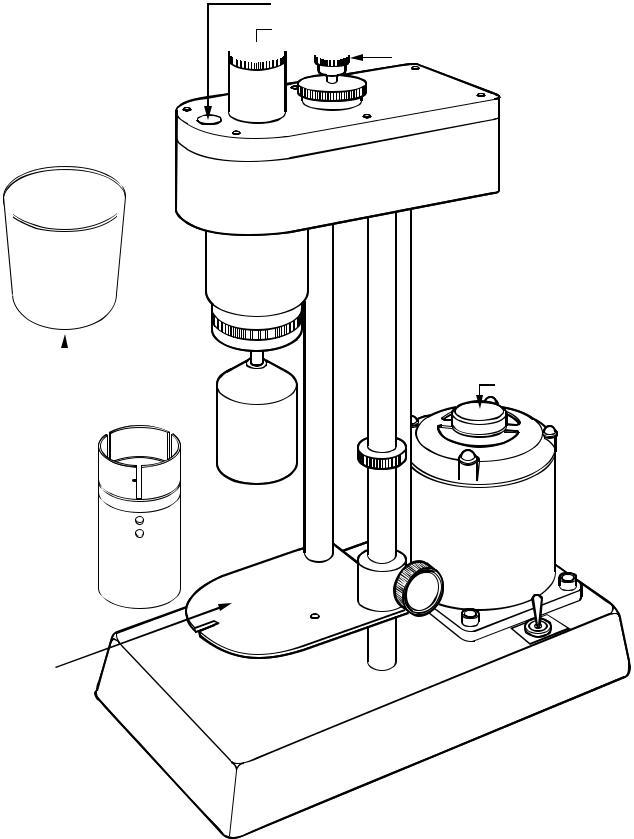
\includegraphics[scale=0.3]{images/marshfunnelvisometer}
\centering 
\caption{A Picture of Marsh Funnel Viscometer}
\end{figure}

\item Gel Strength

The gel strength of the drilling mud can be thought of as the strength of any internal structures which are formed in the mud when it is static. The gel strength of the mud will provide an indication of the pressure required to initiate flow after the mud has been static for some time. The gel strength of the mud also provides an indication of the suspension properties of the mud and hence its ability to suspend cuttings when the mud is stationary . It is measured using rotational viscometer by measuring viscosity at 3rpm and after 10 seconds.

\item Filtration

The filter cake building properties of mud can be measured by means of a filter press. The following are measured during this test :

1. The rate at which fluid from a mud sample is forced through a filter under specified temperature and pressure.

2. The thickness of the solid residue deposited on the filter paper caused by the loss of fluids.

\item pH Determination

The pH of the mud will influence the reaction of various chemicals and must therefore be closely controlled. The pH test is a measure of the concentration of hydrogen ions in an aqueous solution. This can be done either by pH paper or by a special pH meter.

\end{itemize}
 
%mud balance should be added 
%marsh funnel visometer should be added
%pdc and roller cone bits should be added
 
 

\chapter{Mud Conditioning Equipment}

\textbf{Mud Pump:} Sucks mud from the mud pits and pumps it to the drilling apparatus.

\vspace{1em}

\textbf{Shale shaker:}Separates rock cuttings from the mud.

\vspace{1em}

\textbf{Mud pit:} In mud pits drilling mud is mixed and recycled. 

\vspace{1em}

\textbf{Reserve pit:} It collects rock cuttings separated from the mud.

\vspace{1em}

\textbf{Mud-mixing hopper:} In this new mud is mixed and then sent to the mud pits.

\vspace{1em}

\textbf{Desander and Desilter:} In desander sand particles are removed while in desilter small silt particles are removed.

\vspace{2em}

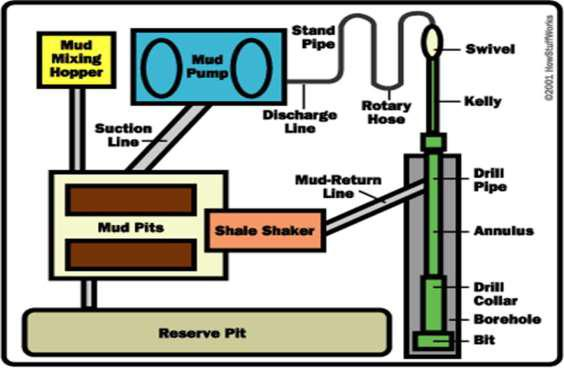
\includegraphics[scale=0.7]{images/Mudconditingequipment}

% Have to insert a figure at the end of this page.

\chapter{Cementing}
	
Cementing operations consist in placing an appropriate cement slurry in 
the annulus between the walls of the hole and the casing that has been run in.
There are several types of cementing jobs and each one meets a particular need.

\vspace{1em}

\textbf{PURPOSE:}

\begin{itemize}

\item Isolating a producing formation from adjacent beds.  
\item Securing the casing mechanically to the borehole walls.
\item Protecting casing from corrosion by fluids contained in the beds that have been drilled.
\item Providing a leak-proof base for safety and control equipment that is installed on the wellhead.
\item Injecting extra cement through the perforations in the casing to consolidate or repair the primary cementing job.
\item Sealing off a depleted productive layer.
\item Isolating a bed from adjacent zones to reduce the per cent of water or gas in oil production.
\item Seal off water influxes.
\item Plug up lost circulation zones.
\item Serve as the basis of a side track.

\end{itemize}


Primary Cementation:

It occurs in 4 stages:

1. The first stage comprises of displacing top plug with pre flush
which is water. The bottom plug cleans up the well by
displacing mud and water occupies its place.

2. Then cement slurry is followed after pre flush is added.

3. Once the pre calculated slurry volume has been added, top plug
is displaced again by spacer (water).

4. Pressure is applied in this process and once the top plug rests
upon bottom plug the bottom plug breaks and tremendous
increase in pressure is noted which tells us the cement job.

CEMENTING THE WELL

\vspace{1em}

After casing, or steel pipe, is run into the well, an L-shaped cementing 
head is fixed to the top of the wellhead to receive the slurry from the pumps. 
Two wiper plugs, or cementing plugs, that sweep the
inside of the casing and prevent mixing: the bottom plug and the top plug.
Keeping the drilling fluids from mixing with the cement slurry, 
the bottom plug is introduced into the well, and cement slurry is pumped into the well behind it. 
The bottom plug is then caught just above the bottom of the wellbore by the float collar, 
which functions as a one-way valve allowing the cement slurry to enter the well.
Then the pressure on the cement being pumped into the well is increased until a diaphragm is broken within the bottom plug,
 permitting the slurry to flow through it and up the outside of the casing string.


%figure of the top plug and bottom plug have to included 

After the proper volume of cement is pumped into the well, a top plug is pumped into 
the casing pushing the remaining slurry through the bottom plug.
 Once the top plug reaches the bottom plug, the pumps are turned off, and the cement is allowed to set.
The amount of time it takes cement to harden is called thickening time or pump ability time. 
For setting wells at deep depths, under high temperature or pressure, as well as in corrosive environments,
 special cements can be employed.


    

\chapter{Drilling Tool Yard Services (DTYS)}

\section*{\textbf{Drill Bits:} }
A drilling bit is the cutting or boring tool which is made
up on the end of the drill string. The bit drills through the rock by
scraping, chipping, gouging or grinding the rock at the bottom of the
hole. Drilling fluid is circulated through passageways in the bit to
remove the drilled cuttings.


There are basically three types of drilling bits:

\begin{enumerate}[(a)]
\item Drag bits
\item Roller Cone bits
\item Diamond bits

\end{enumerate}

\section*{Drag bits:} 

Drag bits were the first bits used in rotary drilling, but are
no longer in common use. A drag bit consists of rigid steel blades
shaped like a fish-tail which rotate as a single unit. These simple
designs were used up to 1900 to successfully drill through soft
formations. The introduction of hard facing to the surface of the
blades and the design of fluid passageways greatly improved its
performance. Due to the dragging/scraping action of this type of bit,
high RPM and low WOB are applied.

%figures of the bits

\section*{\textbf{Roller Cone Bits:}}

Roller cone bits (or rock bits) are still the most
common type of bit used worldwide. The cutting action is provided
by cones which have either steel teeth or tungsten carbide inserts.
These cones rotate on the bottom of the hole and drill hole
predominantly with a grinding and chipping action.
Rock bits are classified as milled tooth bits or insert bits depending
on the cutting surface on the cones.

\vspace{1em}

\section*{\textbf{Diamond bits:}} 

 A new generation of diamond bits
known as polycrystalline diamond compact (PDC)
bits were introduced in the 1980’s. These bits have
the same advantages and disadvantages as natural
diamond bits but use small discs of synthetic
diamond to provide the scraping cutting surface. The
small discs may be manufactured in any size and
shape and are not sensitive to failure along cleavage
planes as with natural diamond. PDC bits have been
run very successfully in many areas around the
world. They have been particularly successful (long
bit runs and high ROP) when run in combination with
turbo drills and oil based mud.

\vspace{1em}

\section*{Blowout Preventers:}

The blowout prevention (BOP)
equipment is the equipment which is used to shut-in a
well and circulates out an influx if it occurs. The
main components of this equipment are the blowout
preventers or BOP's. These are valves which can be
used to close off the well at surface. In addition to the
BOP's the BOP equipment refers to the auxiliary
equipment required to control the flow of the
formation fluids and circulate the kick out safely .

\vspace{1em}


\noindent There are 2 basic types of blowout preventer used for closing in a
well:
\begin{itemize}
\item Annular Preventer
\item Ram Type
\end{itemize}
 
\begin{itemize}
\item \textbf{Annular Preventer:}

 The main component of the
annular BOP is a high tensile strength, circular rubber
packing unit. The rubber is molded around a series of
metal ribs. The packing unit can be compressed
inwards against drill pipe by a piston, operated by
hydraulic power. The advantage of such a well
control device is that the packing element will close
off around any size or shape of pipe. An annular
preventer will also allow pipe to be stripped in (run
into the well whilst containing annulus pressure) and
out and rotated, although its service life is much
reduced by these operations. The rubber packing
element should be frequently inspected for wear and
is easily replaced.Fig 6.1 shows the image of Annular BOP.

\vspace{1em}

\begin{figure}[h]
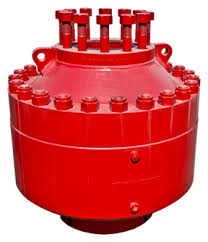
\includegraphics[scale=0.4]{images/bopannular}
\centering
\caption{A Picture of Annular BOP}
\end{figure}

\item \textbf{Ram Type Preventers:}

Ram type preventers derive their name from the twin ram elements which make up their closing mechanism. 
Three types of ram preventers are available: Blind rams - which completely close off the wellbore when 
there is no pipe in the hole.

\vspace{1em}

\end{itemize}

\begin{itemize}

\item Pipe rams - which seal off around a specific size of pipe thus
sealing of the annulus. In 1980 variable rams were made
available by manufacturers. These rams will close and seal on a
range of drill pipe sizes.


\item Shear rams which are the same as blind rams except that they
can cut through drill pipe for emergency shut-in but should only
be used as a last resort. A set of pipe rams may be installed
below the shear rams to support the severed drill string. Fig 6.2 shows the image of Pipe Ram and shear Ram BOP.

\end{itemize}


\begin{figure}[h]
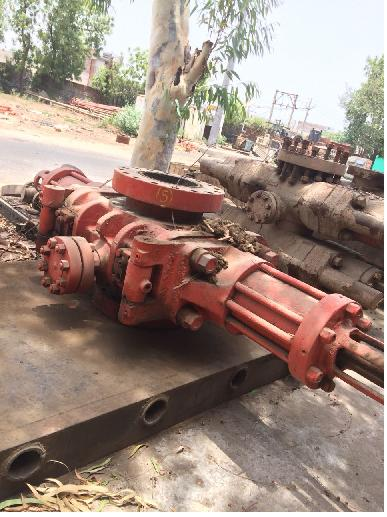
\includegraphics[scale=0.5]{images/shear_ram_BOP}
\centering 
\caption{A Picture of Pipe Ram and Shear Ram BOP}
\end{figure}

\vspace{2em}

An accumulator or Koomey unit is a unit used to hydraulically operate Rams BOP, Annular BOP, 
HCR and some hydraulic equipment. There are several of high pressure cylinders that store gas 
(in bladders) and hydraulic fluid or water under pressure for hydraulic activated systems. 
The primary purpose of this unit is to supply hydraulic power to the BOP stack in order to 
close/open BOP stack for both normal operational and emergency situation. Stored hydraulic in 
the system can provide hydraulic power to close BOP’s in well control operation, therefore, 
kick volume will be minimized. The accumulator should have sufficient volume to close/open 
all preventers and accumulator pressure must be maintained all time. 

\vspace{2em}


\noindent There are 4 main components of the Koomey unit as follows:

\begin{itemize}

\item Accumulators

\item Pumping system (electric and pneumatic pumps)

\item Manifold system

\item Reservoir tank

\end{itemize}



%figures are to be included in this chapter

%noindent should be added in this chapter





\end{document}
